% !TeX spellcheck = en_US

%---------------------------------------------------------------------------------
%--------------------------Set the variables for every client---------------------
%---------------------------------------------------------------------------------
\renewcommand{\hostname}{Example}
\renewcommand{\os}{Linux OS Soft XP}
\renewcommand{\ip}{42.42.42.42}
\renewcommand{\tcpports}{1,2,3}
\renewcommand{\udpports}{23,42}
\renewcommand{\vuln}{CVE-123-42 \glqq Stupid Idiot User\grqq}
\renewcommand{\product}{Human}
%The x-Variables are only used, when root is defined (== root shell)
\renewcommand{\vulnx}{CVE-123-43 \glqq Very Stupid Idiot User Again\grqq} 
\renewcommand{\productx}{Human}
%%%Did you get root? Comment out if you only got low priv access
\def\gotroot{}   %%% Define root if you got root shell
%\undef\gotroot % Else undefine


%----------------------------------------------------------------------------------
%-------------------------------Auto generated content-----------------------------
%----------------------------------------------------------------------------------

\section{\hostname}
\subsection{Service Enumeration}

\begin{table}[h]
	\begin{tabular}{|c|c|}
		\hline
		\multicolumn{2}{|c|}{\textbf{\hostname}}\\\hline\hline
		Type         & Open ports   \\\hline
		TCP          & \tcpports{}  \\\hline
		UDP          & \udpports{}  \\\hline\hline
		\textbf{\os} & \textbf{\ip} \\\hline
	\end{tabular}
	\caption{Service enumeration \hostname}
\end{table}

\subsection{Remote Access Exploitation}

\paragraph{Vulnerability Exploited:}
\vuln

%----------------------------------------------------------------------------------
%-------------------------------Start writing here---------------------------------
%----------------------------------------------------------------------------------
 
\paragraph{Vulnerability Explanation:}
% You can answer the following questions:
% What is the problem?
% What can an attacker do with this vulnerability?
% How did you notice this bug?
% Did you need to change an exploit in order to run it?
% What was the result of the execution?


\paragraph{Vulnerability Fix:}
The publishers of \product{} have issued a patch to fix this known issue.

\paragraph{Severity:}
\textbf{\textcolor{red}{Critical}}

\paragraph{Proof of Concept:} 
Modifications to the existing exploit was needed and is highlighted in red.
\begin{lstlisting}[caption={Exploitation of \hostname}]
SELECT * FROM login WHERE id = **@1 or 1=1@** AND user LIKE "%root%"
In the code section :
*@Green Text@*
**@Red Text@**
***@Blue Text@***
\end{lstlisting}

\begin{figure}[H]
	\centering
	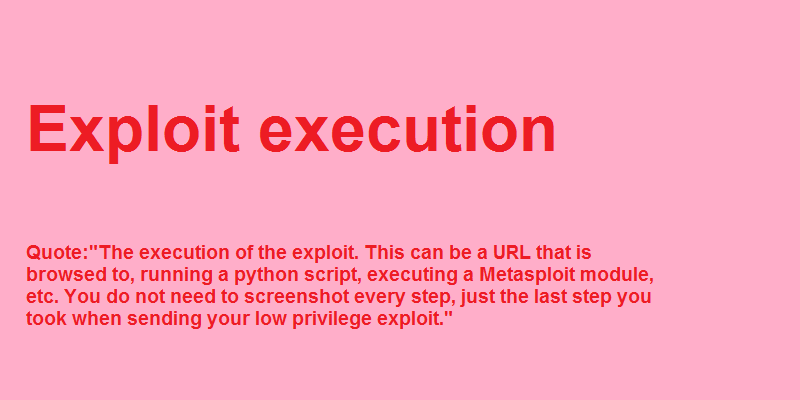
\includegraphics [width=1.0\textwidth]{./hosts/\hostname/1-remote-exploit.png}
	%scale 0.5 bedeutet 50% der originalgröße
	%angle=90 Grafik um 90° drehen
	\caption{Exploitation of \hostname}
\end{figure}

\paragraph{Proof of remote access:} %Print proof for local exploit here
\begin{lstlisting}[caption={Post exploitation of \hostname{} with low privileges}]
hostname && id && ifconfig && cat local.txt
\end{lstlisting}
\begin{figure}[H]
	\centering
	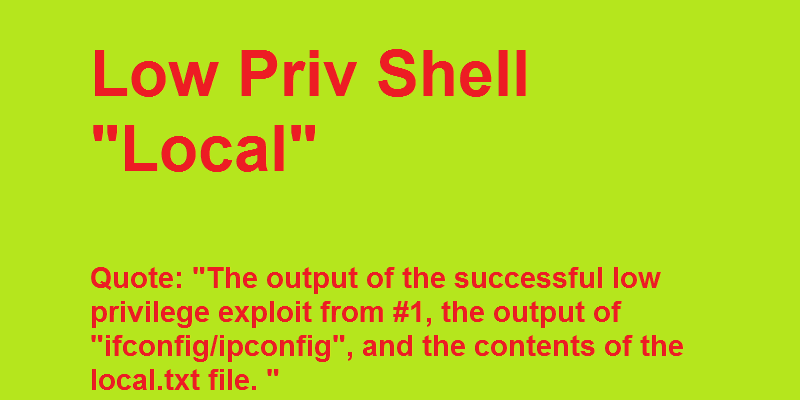
\includegraphics [width=\textwidth]{./hosts/\hostname/2-local.png}
	\caption{Proof of remote access to \hostname}
\end{figure}

%----------------------------------------------------------------------------------
%------------------------------Conditional Privilege Escalation Block--------------
%----------------------------------------------------------------------------------
\ifdefined\gotroot

%----------------------------------------------------------------------------------
%------------------------------Part for Priv escalation----------------------------
%----------------------------------------------------------------------------------
\subsection{Privilege Escalation}

\paragraph{Vulnerability Exploited:}
\vulnx

\paragraph{Vulnerability Explanation:}
% You can answer the following questions:
% What is the problem?
% What can an attacker do with this vulnerability?
% How did you notice this bug?
% Did you need to change an exploit in order to run it?
% What was the result of the execution?


\paragraph{Vulnerability Fix:}
The publishers of \product{} have issued a patch to fix this known issue.

\paragraph{Severity:}
\textbf{\textcolor{red}{Critical}}

\paragraph{Proof of Concept:} 
Modifications to the existing exploit was needed and is highlighted in red.
\begin{lstlisting}[caption={Exploitation of \hostname}]
SELECT * FROM login WHERE id = **@1 or 1=1@** AND user LIKE "%root%"
In the code section :
*@Green Text@*
**@Red Text@**
***@Blue Text@***
\end{lstlisting}

\begin{figure}[H]
	\centering
	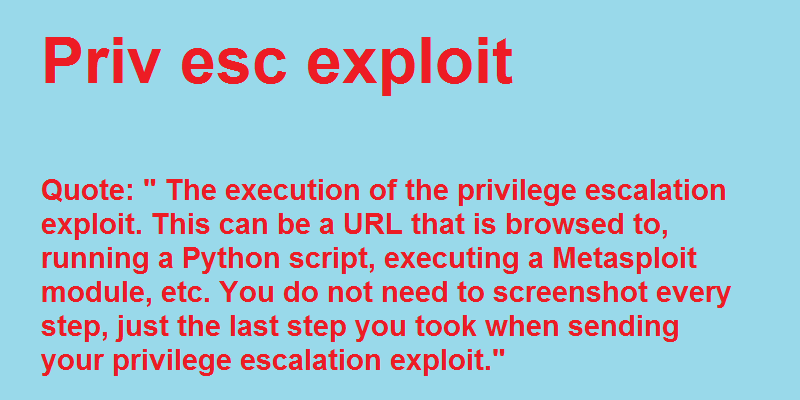
\includegraphics [width=1.0\textwidth]{./hosts/\hostname/3-privesc-exploit.png}
	\caption{Privilege escalation exploit of \hostname}
\end{figure}

\paragraph{Proof of successful privilege escalation:}
\begin{lstlisting}[caption={Post exploitation of \hostname}]
hostname && id && ifconfig && cat proof.txt
\end{lstlisting}

\begin{figure}[H]
	\centering
	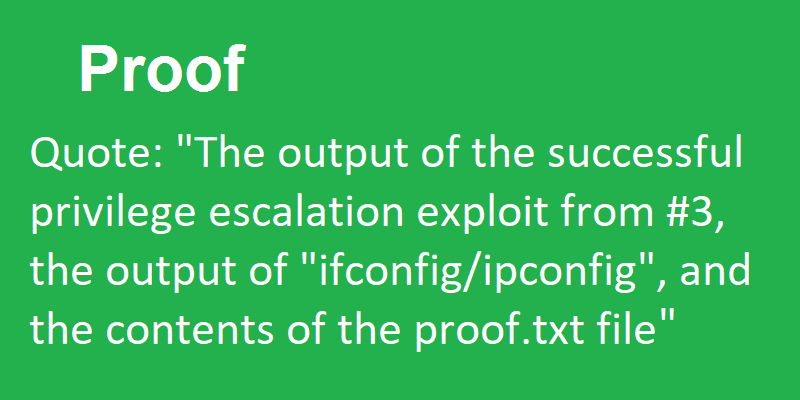
\includegraphics [width=\textwidth]{./hosts/\hostname/4-proof.png}
	\caption{Proof of successful privilege escalation on \hostname}
\end{figure}
\fi % End of if-block
%----------------------------------------------------------------------------------
%--------------------------------------End of Priv Esc Block-----------------------
%----------------------------------------------------------------------------------


